
\section{Solução Ponte H}

Para o projeto Green House, foi necessária a confecção de uma ponte H para controle da rotação do motor. Foi realizada uma simulação no Proteus®, a fim de garantir a tensão de 12V para carga, a funcionalidade do circuito é demonstrada também a entrada do controlador de operações (representado pelos 3,3V):

\begin{figure}[H]
	\centering
	\includegraphics[width=14cm]{figuras/simulacaoPonteH.png}
	\caption{Simulação da ponte H com acionamento em Q1 e Q4. Fonte: Proteus*.}
	\label{simulação ponte H}
\end{figure}

\begin{figure}[H]
	\centering
	\includegraphics[width=14cm]{figuras/simulacaoPonteH2.png}
	\caption{Simulação da ponte H com acionamento em Q2 e Q3. Fonte: Proteus*.}
	\label{simulação ponte H 2}
\end{figure}

O microcontrolador utilizado é uma Raspberry que trabalha com 3,3V e tem limitação na corrente de 50mA, quando utilizadas todas as suas entradas. Assim, para que essa restrição seja limitada, no nó de conexão entre o transístor e o controlador, a corrente foi limitada a 0,005mA. Para isso ocorrer, é necessário o uso de resistências de 520$\Omega$, como demonstrado a seguir:

\begin{center}
	
	$\frac{V_{cc} - V_{be}}{R}$ = $l_{b}$ \\
	$\frac{3,3 - 0,7}{R}$ = 0,005\\
	R = 520$\Omega$\\
	$I_{ce}$ = 1000 $\Omega$ * 0,005 = 5 \textit{A}
	
\end{center}

Onde,

\begin{itemize}
	
\item Ib = corrente que aciona o transistor;

\item R = resistências que serão utilizadas para controle da corrente Ib;

\item $I_{ce}$ = corrente disponível à carga;

\item ${V_{cc} - V_{be}}$ = diferença de tensão entre o controlador e o transístor.

\end{itemize}

A corrente $I_{ce}$ é multiplicada por 1000 devido ao transistor TIP. Para a construção dessa ponte H, serão necessários:

\begin{itemize}
	
	\item 2 transístores Darlington TIP 120;
	\item 2 transístores Darlington TIP 125;
	\item 4 resistências de 520$\Omega$;
	\item 1 placa furada;
	\item 3 Borne Conector 2 vias - entradas PCI
	
\end{itemize}

As especificações dos transistores e resistências estão em anexo.

\section{Solução Plantário}

O sistema contém uma bomba que eleva a água do reservatório para 40 cm acima do mesmo, onde estarão os canos. Os canos estão dispostos com uma angulação que permite que o fluído percorra o cano pela ação da gravidade. Assim, não é preciso fazer cálculos de perdas de cargas das raízes do substrato. A potência pelo fluxo mássico é dado pela variação de energia na entrada e saída da bomba. De acordo com Silva \cite{SILVA}, a vazão volumétrica para um sistema de hidroponia é de 2L/min, ou seja, 3,33.$10^{-5}$ $m^3$. Como representado a seguir, há a variação de energia de pressão, energia cinética e energia potencial:

\begin{center}
	${\displaystyle\frac{W}{m} = (\frac{P2}{\rho} + \frac{V2^2}{2} + gH2) - (\frac{P1}{\rho} + \frac{V1^2}{2} + gH1)}$	
\end{center}

Onde,

$W$ = potência consumida (W/s);

$m$ = fluxo mássico (kg/s);

$P2$ = pressão no ponto 2;

$\rho$ = massa específica da água (kg/m³);

$V2$ = velocidade no ponto 2 (m/s)

$H2$ = altura no ponto 2 (m);

$g$ = gravidade (m²/s);

$P1$ = pressão no ponto 1;

$V1$ = velocidade no ponto 1 (m/s);

$H1$ = altura no ponto 1 (m);

Considera-se que não há variação de altura considerável entre a entrada e saída da bomba. Assim, não há variação de energia potencial. Considera-se também que não há variação de energia cinética no sistema (V2 aproximadamente igual a V1). Nota-se, então, que o sistema fornece apenas energia de pressão, essa mesma que torna possível a elevação da coluna de água. Dessa forma:

\begin{center}
	\large
	${\displaystyle \frac{W}{m} = H_g + \frac{P2-P1}{\rho}+ \frac{\Delta_p}{\rho g}}$
\end{center}

A perda de pressão distribuída é dada por: 

\begin{center}
	\large
	${\displaystyle \Delta P = f \frac{L}{D} \frac{1}{2} \frac{Q^2}{A^2} \rho}$
\end{center}

Onde,

$f$ = fator de atrito;

$L$ = comprimento do escoamento (m) ;

$D$ = diâmetro;

$\rho$ = massa específica da água (kg/m³);

$A$ = área do escoamento ($m^2$);

$Q$ = vazão volumétrica ($m^3$/s).

O fator de atrito é dado por:
 
$f$ = 0,005 $\left [ 1 + (20000 \frac{\epsilon}{Dr} + \frac{10^6}{Re} )^{1/3} \right ]$

Onde $\epsilon$ é a rugosidade do material da tubulação de escoamento. O material selecionado foi o polietileno, cujo fator de atrito é dado por 0,0015mm. O diâmetro do tubo (Dr) é de 0,005m. A imagem a seguir reporta a mangueira já conectado aos tubos. 

\begin{figure}[H]
	\centering
	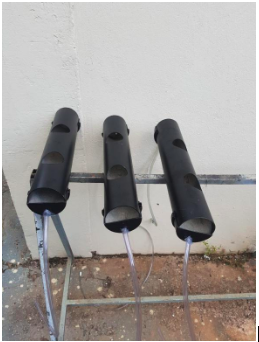
\includegraphics[width=10cm]{figuras/tubos_plantario.png}
	\caption{Tubos do plantário. Fonte própria.}
	\label{tubos_plantario}
\end{figure}

O número de Reynolds é dado por:

$R$ = $\frac{4Q}{\Pi Dr v}$ = 8462,85 > 2400 (escoamento turbulento)

Dessa forma, o fator de atrito é de 0,106. E a perda de carga do sistema é de 0,2397 Pa. Assim, a potência necessária para o sistema é dada por:

$P3 - P2 = pgH = P2 - P1$\\

$W = mgH + dH = pQgH + dh = 1000 * 3,33 * 10^{-5} * 10 * 0,4 + 2,44E - 5$\\

$W \approx 0,1333 W $

O dimensionamento da bomba não condiz com o que realmente foi utilizado, pois as bombas comerciais são tabeladas. Cada fornecedor de bombas trabalha com um rendimento específico do seu produto. O fornecedor de bomba Sarlobetter®, por exemplo, traz a curva característica de seus produtos. Nota-se que, quando há uma altura de 0,5m de elevação a vazão real para a bomba de 520L/h decai para 380L/h. Dessa forma, para uma vazão de 120L/h e uma elevação de 0,4m, bomba ideal é a S300 (300L/h) visto que com o aumento da coluna a ser vencida, a vazão decai e a bomba deixa de operar com sua vazão de projeto.  

\begin{figure}[H]
	\centering
	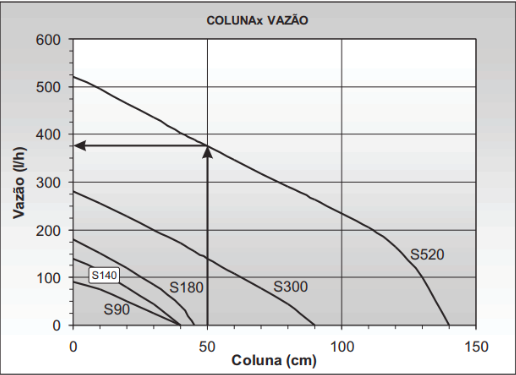
\includegraphics[width=10cm]{figuras/curva_moto.png}
	\caption{Curva característica da moto bomba.}
	\label{curva_moto}
\end{figure}

A fim de reduzir os custos, serão utilizadas bombas que os integrantes já possuíam. As bombas são de 220L/h e 4W, compradas após as anteriores terem sido queimadas.
O reservatório contém também um compressor de ar com a finalidade de auxiliar no processo de dissolução dos nutrientes. Como seu fim é apenas \textit{mixer}, sua seleção foi feita a partir do menor preço de mercado. O compressor que é utilizado é mostrado a seguir:


\begin{figure}[H]
	\centering
	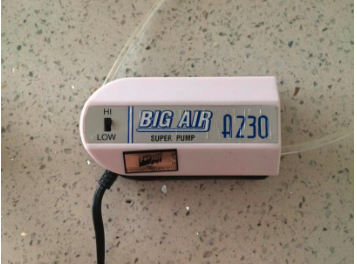
\includegraphics[width=5cm]{figuras/compressor.png}
	\caption{Compressor de ar. Fonte própria}
	\label{compressor}
\end{figure}

\section{Solução Alimentação}

Primeiramente, tentou-se construir uma fonte baseada em um regulador de tensão LM 7812 e um regulador de corrente com TIPs 122. Quando conectado a uma carga, a tensão caia consideravelmente. Depois de vários testes, desconsiderou-se essa disposição. As cargas pontualmente não passam de 1A, sendo essa a corrente limite do regulador LM 7812 (\textit{datasheet} em anexo). Dessa forma, foi desenvolvida uma fonte com dois reguladores de tensão, fornecendo assim duas saídas de 12V e 1A. Adicionou-se a uma delas um \textit{step down}, para que a tensão fosse reduzida até 5V. A carga a ser alimentada pela fonte desenvolvida consistiu em:


\begin{table}[H]
	\centering
	\caption{Tabela Tensão-Corrente}
	\label{table-tensao}
	\begin{tabular}{|l|l|}
		\hline
		\textbf{Tensão (V)}                                    & \textbf{Corrente(mA)} \\ \hline
		\textbf{5V}                                            &                       \\ \hline
		Sensor PH                                              & 10                    \\ \hline
		Sensor PCF8591                                         & 50                    \\ \hline
		\textbf{12V}                                           &                       \\ \hline
		Motor da gaveta                                        & 1000                  \\ \hline
		\begin{tabular}[c]{@{}l@{}}Cooler\\  12cm\end{tabular} & 120                   \\ \hline
		\begin{tabular}[c]{@{}l@{}}Cooler\\  8cm\end{tabular}  & 80                    \\ \hline
		Total                                                  & 1260                  \\ \hline
	\end{tabular}
\end{table}

Para atender essas especificações. Foi simulada uma fonte simples no software Proteus.  A resistência utilizada simula a carga.

\begin{figure}[H]
	\centering
	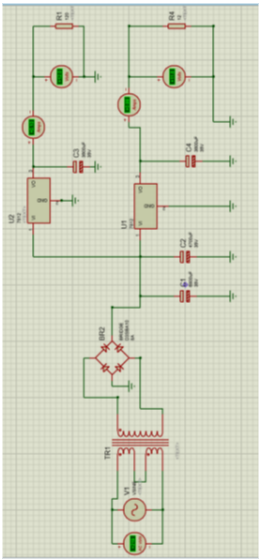
\includegraphics[width=5cm]{figuras/fonte_funcionamento.png}
	\caption{Fonte em funcionamento.}
	\label{fonte_funcionamento}
\end{figure}

\begin{figure}[H]
	\centering
	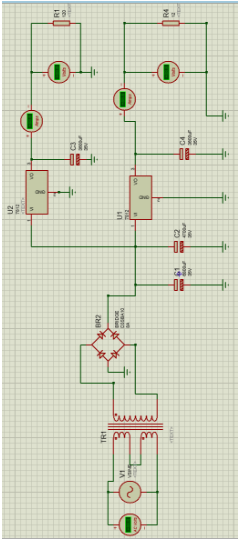
\includegraphics[width=5cm]{figuras/simulacao_fonte.png}
	\caption{Simulação de fonte.}
	\label{simulacao_fonte}
\end{figure}

Nota-se que foram utilizados:

\begin{itemize}
	
	\item 1 transformador 220/20V;
	\item 1 ponte retificadora 8A;
	\item 1 capacitor 6800 $\mu$F 35V; 
	\item 2 capacitorres 3800 $\mu$F 35V;
	\item 1 capacitor 4700 $\mu$F 35V;
	\item 3 bornes;
	\item 1 step down;
	\item 1 fusível.
	
\end{itemize}

\section{Solução Iluminação}

A alface, por não ter em seu ciclo, flores, frutos e outras estruturas mais complexas, permite o crescimento com uma boa faixa de iluminação para o período de 16 horas de luz,variando entre 30W, onde o produto final teria um tamanho reduzido mas mantendo a qualidade das folhas e 80W no qual acima disso teria um excedente de iluminação causando queimaduras nas pontas das folhas e inibindo o crescimento.
Dessa forma foi programado 3 bocais nos quais seriam possíveis tanto uma estrutura mais econômica  ao utilizar 1 LED especializado na proporção de 15 leds vermelhos para 7 azuis e com emissão de infravermelho e ultravioleta com 2 lâmpadas led comum , tanto  quanto uma configuração maximizada utilizando 3 LEDs especiais .
O posicionamento foi determinado com base em gráfico de densidade de iluminação na qual o posicionamento alinhado na horizontal com 10cm de distância da borda proporcionou melhor igualdade de distribuição utilizando a fórmula de uma Cardioide.

$y=1+cos(\theta).$\\
$cos(\theta)=cat.adj/hipotenusa.$\\
$cat.adj=altura lampada teto.$\\
$Hipotenusa=distância ponto-lâmpada.$\\

Juntamente com a parte reflexiva instalada nas paredes e teto da estufa na qual melhora o aproveitamento da luz pela planta.

\begin{figure}[H]
	\centering
	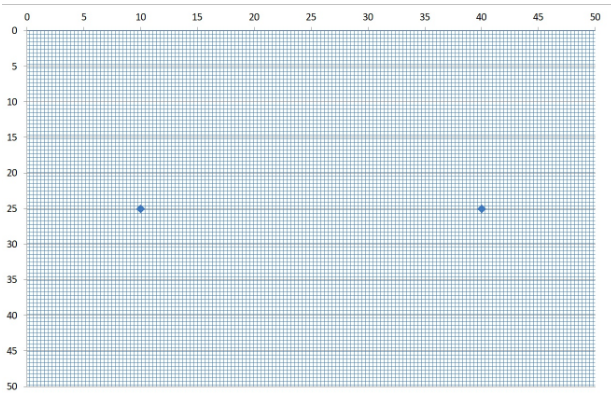
\includegraphics[width=5cm]{figuras/posicao_lampadas.png}
	\caption{Posição das lâmpadas.}
	\label{posicao_lampadas}
\end{figure}

\begin{figure}[H]
	\centering
	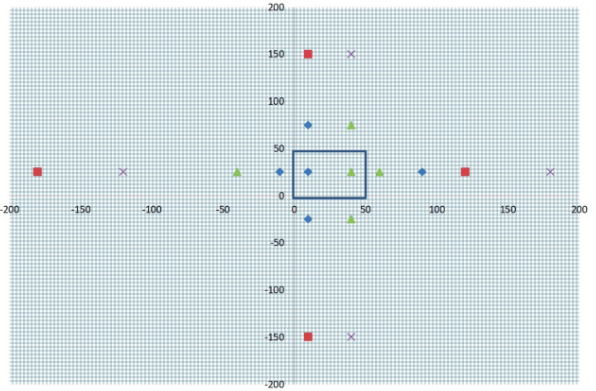
\includegraphics[width=5cm]{figuras/reflexos_lampadas.png}
	\caption{Reflexos e reflexões das lâmpadas.}
	\label{reflexos_lampadas}
\end{figure}

\begin{figure}[H]
	\centering
	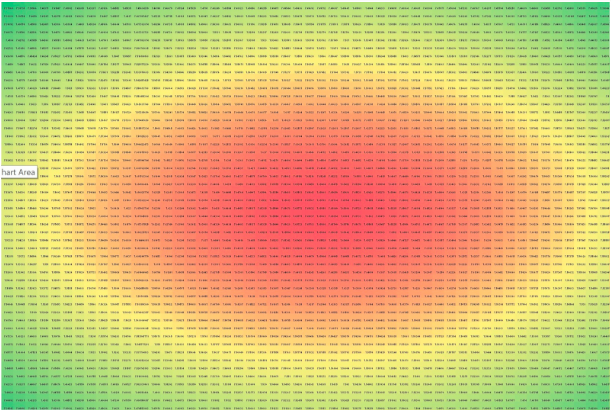
\includegraphics[width=5cm]{figuras/grafico_luminosa.png}
	\caption{Gráfico de densidade luminosa.}
	\label{grafico_luminosa}
\end{figure}